		\section{Nombre: Viento temporal}\label{obs.vientoT}
	\subsection{Descripción}
	Ráfaga de viento. Impulsa al jugador de manera horizontal, dependiendo del nivel lo empujara hacia la izquierda o hacia la derecha. Su efecto no es constante, se activa y desactiva de manera periódica estando activo durante un tiempo determinado y desactivándose por otro tiempo determinado; los tiempos de actividad e inactividad pueden no ser los mismos. Para superar este obstáculo el jugador deberá aprovechar los tiempos de inactividad y cruzar la zona donde aparece la ráfaga.
	\subsection{Esquema}
	Ver figura \ref{fig:vientoT}.
	\begin{figure}
		\centering
		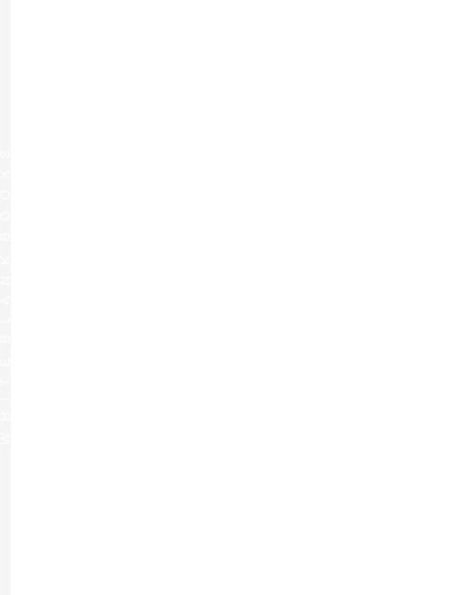
\includegraphics[height=0.2 \textheight]{Imagenes/vientoT}
		\caption{Dirección que el viento toma respecto al jugador.}
		\label{fig:vientoT}
	\end{figure}